\section{بخش اول: فراخوانی تصویر و آستانه‌گذاری ساده}

\begin{stepbox}
\field{هدف این بخش (بخش ۰ و ۱)}{
بارگذاری تصویر اسکن شده با مقادیر ۸ بیتی و بررسی امکان جداسازی متن از پس‌زمینه در شرایط روشنایی غیریکنواخت، تنها با استفاده از تکنیک آستانه‌گذاری ساده (\lr{Simple Thresholding}) با مقادیر آستانه‌ی ۶۰، ۱۲۰ و ۱۸۰.
}
\end{stepbox}

\subsection{کد پیاده‌سازی و منطق آن}
به جای آوردن کدهای تکراریِ خواندن و ذخیره‌ی تصویر، تمرکز اصلی ما بر روی هسته‌ی پردازشیِ این بخش یعنی تابع آستانه‌گذاری است:

\begin{codebox}[\lr{Simple Thresholding Core}]
\begin{lstlisting}[language=Python]
# Apply simple thresholding with value T
ret, thresh_img = cv2.threshold(img, T, 255, cv2.THRESH_BINARY)
\end{lstlisting}
\end{codebox}

\textbf{توضیح کد:}
تابع \lr{\texttt{cv2.threshold}} در کتابخانه \lr{\texttt{OpenCV}}، تک‌تک پیکسل‌های تصویر را با مقدار آستانه (\lr{T}) مقایسه می‌کند. پارامتر \lr{\texttt{cv2.THRESH\_BINARY}} به این تابع دستور می‌دهد که اگر مقدار روشنایی پیکسلی از حد آستانه بیشتر بود، آن را به سفید مطلق (۲۵۵) و اگر کمتر بود، به سیاه مطلق (۰) تبدیل کند.

\subsection{خروجی‌های تصویری و تحلیل دقیق آن‌ها}
تصویر اصلی دارای سایه‌ای در سمت چپ است که باعث توزیع نامناسب روشنایی روی کاغذ شده است. خروجی‌های اجرای کد بالا برای سه آستانه متفاوت در شکل \ref{fig:part1_thresh} آورده شده است.

\begin{figure}[h!]
    \centering
    \begin{subfigure}{0.31\textwidth}
        \centering
        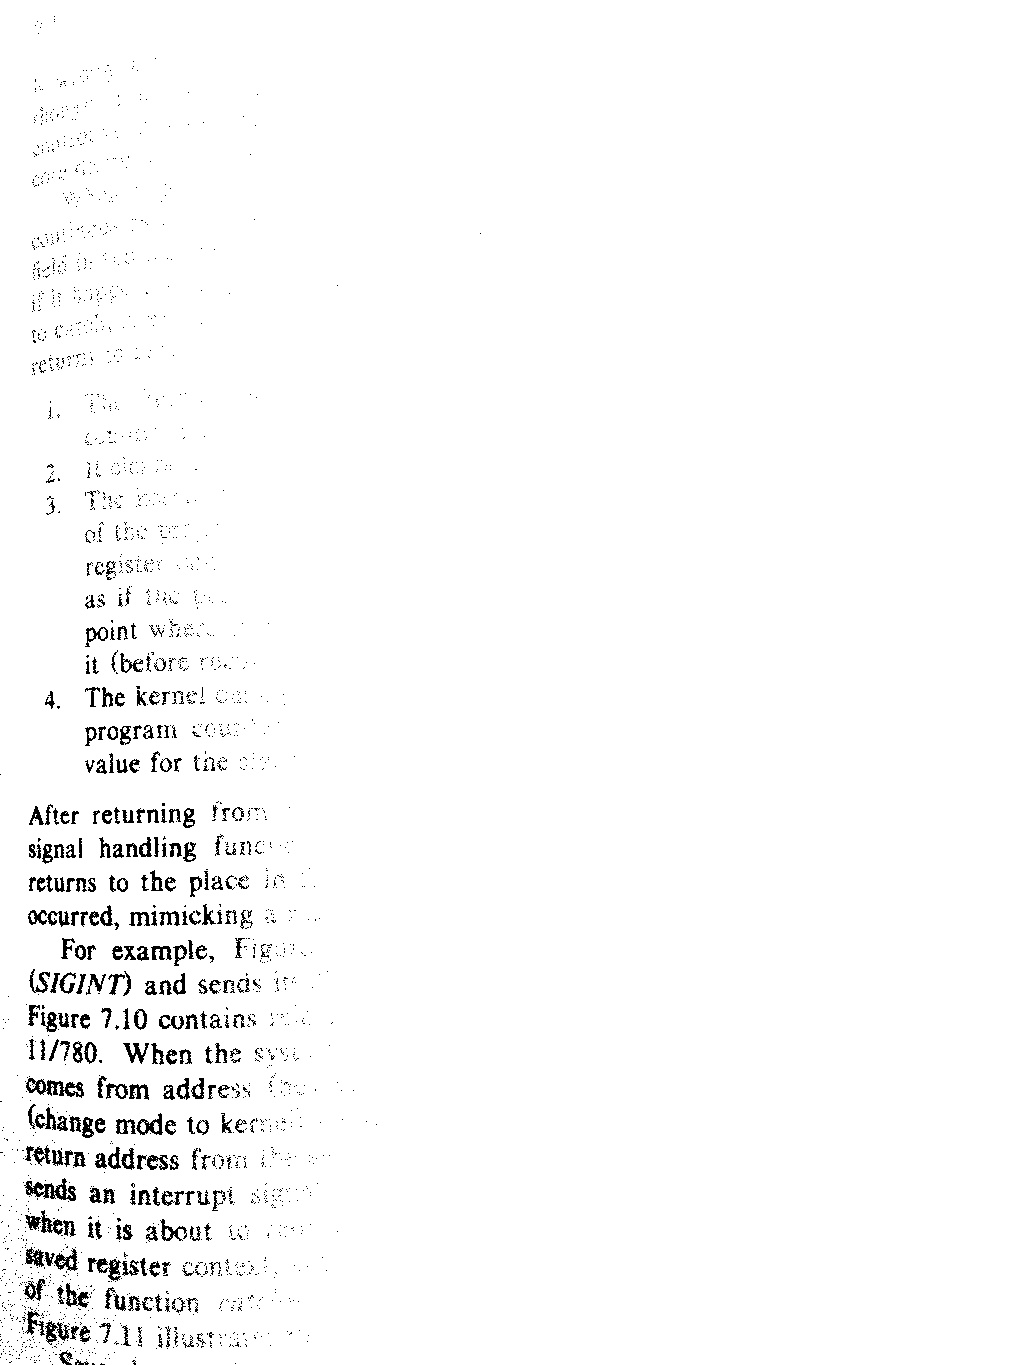
\includegraphics[width=\linewidth]{images/thresh_60.jpg}
        \caption{آستانه = ۶۰}
    \end{subfigure}
    \hfill
    \begin{subfigure}{0.31\textwidth}
        \centering
        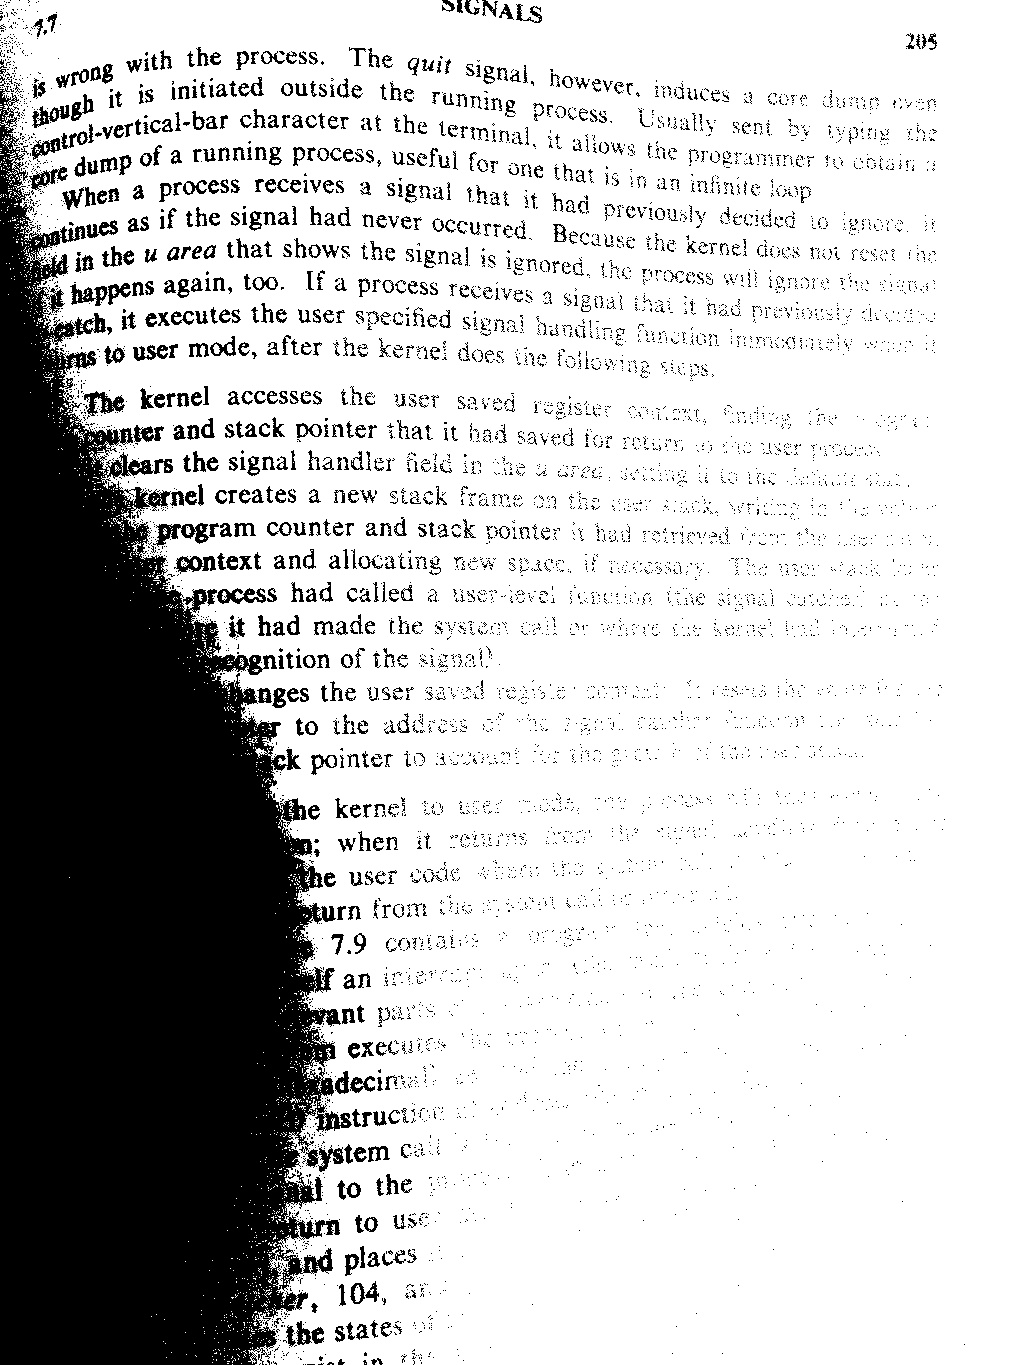
\includegraphics[width=\linewidth]{images/thresh_120.jpg}
        \caption{آستانه = ۱۲۰}
    \end{subfigure}
    \hfill
    \begin{subfigure}{0.31\textwidth}
        \centering
        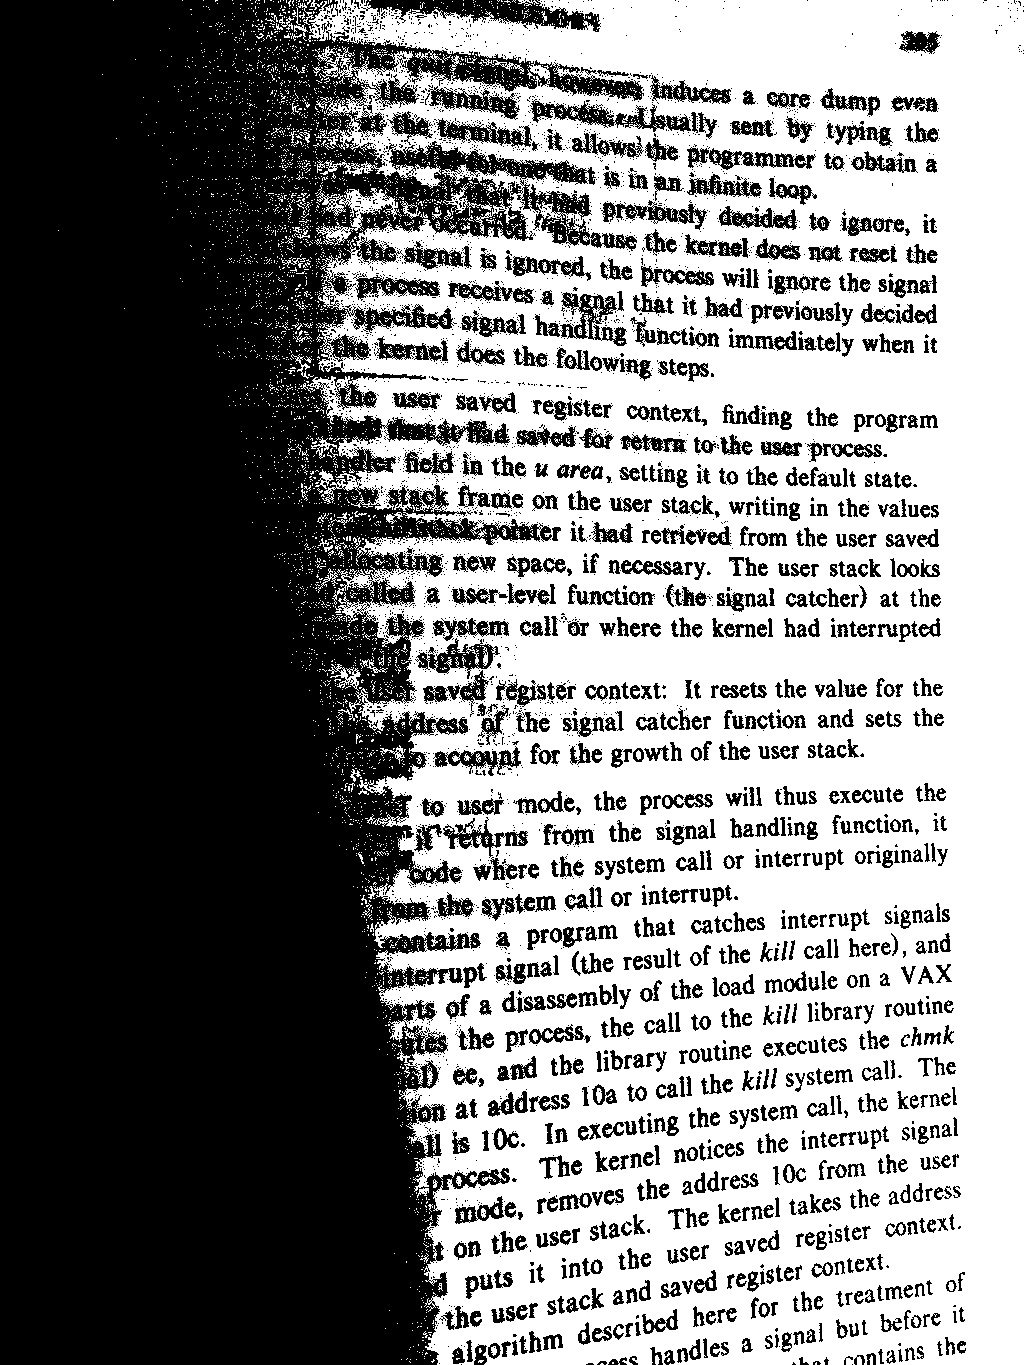
\includegraphics[width=\linewidth]{images/thresh_180.jpg}
        \caption{آستانه = ۱۸۰}
    \end{subfigure}
    \caption{نتایج آستانه‌گذاری ساده با سطوح مختلف}
    \label{fig:part1_thresh}
\end{figure}

\textbf{کالبدشکافی و تحلیل تصاویر خروجی:}
با دقت در خروجی‌های به دست آمده، رفتار تابع آستانه‌گذاری در مواجهه با روشنایی متغیر به شکل زیر تحلیل می‌شود:
\begin{itemize}
    \item \textbf{تصویر با آستانه ۶۰ (\lr{T = 60}):} از آنجایی که عدد ۶۰ به رنگ سیاه بسیار نزدیک است، تقریباً تمام پیکسل‌های سمت راست تصویر (اعم از جوهر متن و خود کاغذ) مقداری بالاتر از ۶۰ داشته و کاملاً سفید شده‌اند. تنها تاریک‌ترین بخش‌های سایه در لبه‌ی سمت چپ توانسته‌اند شرط تاریک‌تر بودن از ۶۰ را برآورده کنند و سیاه بمانند.
    \item \textbf{تصویر با آستانه ۱۲۰ (\lr{T = 120}):} این عدد در میانه‌ی طیف خاکستری (\lr{Grayscale}) قرار دارد. در سمت راست، متن‌ها تا حدودی خوانا شده‌اند، اما سایه‌ی روی کاغذ در سمت چپ آن‌قدر غلیظ است که روشناییِ خودِ پس‌زمینه (کاغذ) در آن قسمت کمتر از ۱۲۰ بوده و کاملاً سیاه شده است؛ در نتیجه متن در دل تاریکی بلعیده شده است.
    \item \textbf{تصویر با آستانه ۱۸۰ (\lr{T = 180}):} این آستانه به رنگ سفید نزدیک است. در قسمت راستِ تصویر، متن‌ها با وضوح و ضخامت بالا استخراج شده‌اند، اما در قسمت‌های چپ و حتی مرکز، روشناییِ کاغذ به دلیل سایه به زیر ۱۸۰ افتاده و بخش عظیمی از پس‌زمینه به عنوان نقطه تاریک شناسایی و سیاه شده است.
\end{itemize}

\subsection{پاسخ به سوالات تمرین}
\textbf{آیا در هیچ کدام از این سه حالت متن و پس‌زمینه تا حد خوبی از یکدیگر جدا شده‌اند؟} \\
خیر. همان‌طور که در تحلیل فوق تشریح شد، به دلیل وجود سایه، روشنایی در قسمت‌های مختلف تصویر یکنواخت نیست و هیچ‌یک از تصاویر نتوانستند تفکیک مناسبی ارائه دهند.

\textbf{آیا سطح آستانه بهتری می‌توان پیدا کرد؟} \\
خیر، هیچ «سطح آستانه سراسری» (\lr{Global Threshold}) واحدی نمی‌تواند کل این تصویر را به درستی تفکیک کند. مشکل اساسی این است که مقدار روشنایی پس‌زمینه در قسمتِ سایه‌دار، به مراتب تاریک‌تر از مقدار روشناییِ خودِ متن در قسمتِ روشن تصویر است. لذا استفاده از روش‌های محلی یا تخمین پس‌زمینه الزامی است.